\documentclass[12pt,a4paper]{report}
\usepackage[utf8]{inputenc}
\usepackage[T1]{fontenc}
\usepackage[english]{babel}
\usepackage[top=2.5cm,bottom=2.5cm,left=2.5cm,right=2.5cm]{geometry}
\usepackage{amsmath,amssymb,amsthm}
\usepackage{graphicx}
\usepackage{tikz}
\usepackage{pgfplots}
\pgfplotsset{compat=1.18}
\usepackage{tcolorbox}
\usepackage{enumitem}
\usepackage{hyperref}
\usepackage{bookmark}
\usepackage{fancyhdr}
\usepackage{titlesec}

% Theorem environments
\theoremstyle{definition}
\newtheorem{definition}{Definition}[section]
\newtheorem{example}{Example}[section]
\theoremstyle{plain}
\newtheorem{theorem}{Theorem}[section]
\newtheorem{property}{Property}[section]
\theoremstyle{remark}
\newtheorem{remark}{Remark}[section]

% Custom boxes
\tcbuselibrary{theorems,skins,breakable}
\newtcolorbox{keypoint}{
    colback=blue!5!white,
    colframe=blue!75!black,
    fonttitle=\bfseries,
    title=Key Point,
    breakable
}
\newtcolorbox{warning}{
    colback=red!5!white,
    colframe=red!75!black,
    fonttitle=\bfseries,
    title=Common Mistake,
    breakable
}
\newtcolorbox{formula}{
    colback=green!5!white,
    colframe=green!60!black,
    fonttitle=\bfseries,
    title=Formula,
    breakable
}
\newtcolorbox{algorithmbox}{
    colback=purple!5!white,
    colframe=purple!60!black,
    fonttitle=\bfseries,
    title=Algorithm,
    breakable
}

% Header/Footer
\pagestyle{fancy}
\fancyhf{}
\fancyhead[L]{\leftmark}
\fancyhead[R]{Mathematics 101}
\fancyfoot[C]{\thepage}

\title{\Huge\textbf{Numerical Analysis}\\[0.5cm]
\Large Mathematics 101 --- Study Material\\[0.3cm]
\normalsize Computational Methods for Mathematical Problems}
\author{SOLTANI Achraf\\
\texttt{achraf.soltani@pm.me}}
\date{\today}

\begin{document}

\maketitle

\chapter*{About This Course}
\addcontentsline{toc}{chapter}{About This Course}

This study material covers \textbf{Numerical Analysis}, the branch of mathematics concerned with developing and analyzing algorithms for obtaining numerical solutions to mathematical problems.

\textbf{Course Structure:}
\begin{itemize}
    \item \textbf{Chapter 1:} Errors and Approximations --- Sources of error, floating-point arithmetic
    \item \textbf{Chapter 2:} Root Finding Methods --- Bisection, Newton-Raphson, Secant, Fixed-Point
    \item \textbf{Chapter 3:} Interpolation --- Lagrange, Newton's Divided Differences, Splines
    \item \textbf{Chapter 4:} Numerical Differentiation and Integration --- Finite differences, Trapezoidal, Simpson's
    \item \textbf{Chapter 5:} Linear Systems --- Gaussian Elimination, LU Decomposition, Iterative Methods
    \item \textbf{Chapter 6:} Numerical Solutions of ODEs --- Euler's Method, Runge-Kutta Methods
\end{itemize}

\textbf{Learning Outcomes:} By the end of this course, you will be able to:
\begin{itemize}
    \item Understand and quantify different types of numerical errors
    \item Apply root-finding algorithms to solve nonlinear equations
    \item Construct interpolating polynomials and understand their limitations
    \item Approximate derivatives and integrals numerically
    \item Solve systems of linear equations using direct and iterative methods
    \item Approximate solutions to ordinary differential equations
\end{itemize}

\tableofcontents
\newpage

%=============================================================================
%=============================================================================
\chapter{Errors and Approximations}
%=============================================================================
%=============================================================================

\section{Introduction to Numerical Errors}

Numerical methods provide \textit{approximate} solutions to mathematical problems. Understanding the sources and types of errors is crucial for assessing the reliability of computed results.

\subsection{Types of Errors}

\begin{definition}[Absolute Error]
The \textbf{absolute error} is the magnitude of the difference between the exact value $x$ and the approximate value $\tilde{x}$:
\[
E_a = |x - \tilde{x}|
\]
\end{definition}

\begin{definition}[Relative Error]
The \textbf{relative error} measures the error relative to the exact value:
\[
E_r = \frac{|x - \tilde{x}|}{|x|} \quad (x \neq 0)
\]
Often expressed as a percentage: $E_r \times 100\%$
\end{definition}

\begin{example}
If the exact value is $x = 3.14159$ and the approximation is $\tilde{x} = 3.14$:
\begin{align*}
E_a &= |3.14159 - 3.14| = 0.00159\\
E_r &= \frac{0.00159}{3.14159} \approx 0.000506 = 0.0506\%
\end{align*}
\end{example}

\begin{keypoint}
Relative error is often more meaningful than absolute error. An error of 1 meter is significant when measuring a room, but negligible when measuring the distance to the Moon.
\end{keypoint}

\subsection{Sources of Error}

\begin{enumerate}
    \item \textbf{Round-off Error}: Due to finite precision of computer arithmetic
    \item \textbf{Truncation Error}: Due to approximating infinite processes with finite ones (e.g., truncating Taylor series)
    \item \textbf{Input Error}: Errors in the initial data or measurements
    \item \textbf{Human Error}: Programming mistakes, incorrect formulas
\end{enumerate}

%-----------------------------------------------------------------------------
\section{Floating-Point Arithmetic}
%-----------------------------------------------------------------------------

\subsection{Floating-Point Representation}

\begin{definition}[Floating-Point Number]
A floating-point number is represented as:
\[
x = \pm m \times \beta^e
\]
where:
\begin{itemize}
    \item $m$ is the \textbf{mantissa} (significand)
    \item $\beta$ is the \textbf{base} (usually 2 or 10)
    \item $e$ is the \textbf{exponent}
\end{itemize}
\end{definition}

\begin{example}
In base 10: $3.14159 \times 10^2 = 314.159$

In normalized form: $0.314159 \times 10^3$
\end{example}

\subsection{Machine Epsilon}

\begin{definition}[Machine Epsilon]
The \textbf{machine epsilon} $\epsilon_m$ is the smallest positive number such that:
\[
\text{fl}(1 + \epsilon_m) > 1
\]
where $\text{fl}(\cdot)$ denotes the floating-point representation.
\end{definition}

For IEEE 754 double precision: $\epsilon_m \approx 2.2 \times 10^{-16}$

\begin{warning}
Never test floating-point numbers for exact equality! Instead of \texttt{if (a == b)}, use \texttt{if (|a - b| < tolerance)}.
\end{warning}

\subsection{Loss of Significance}

\begin{definition}[Catastrophic Cancellation]
\textbf{Catastrophic cancellation} occurs when subtracting two nearly equal numbers, causing significant digits to be lost.
\end{definition}

\begin{example}
Computing $\sqrt{x+1} - \sqrt{x}$ for large $x$:

For $x = 10^8$: Both terms $\approx 10^4$, but their difference is $\approx 5 \times 10^{-5}$.

\textbf{Better formula:} Rationalize to avoid subtraction:
\[
\sqrt{x+1} - \sqrt{x} = \frac{(\sqrt{x+1} - \sqrt{x})(\sqrt{x+1} + \sqrt{x})}{\sqrt{x+1} + \sqrt{x}} = \frac{1}{\sqrt{x+1} + \sqrt{x}}
\]
\end{example}

%-----------------------------------------------------------------------------
\section{Significant Figures}
%-----------------------------------------------------------------------------

\begin{definition}[Significant Figures]
The \textbf{significant figures} of a number are all digits except:
\begin{itemize}
    \item Leading zeros (e.g., 0.0045 has 2 significant figures)
    \item Trailing zeros used only as placeholders (ambiguous without scientific notation)
\end{itemize}
\end{definition}

\begin{property}[Significant Figures in Arithmetic]
\begin{itemize}
    \item \textbf{Addition/Subtraction}: Result has as many decimal places as the least precise input
    \item \textbf{Multiplication/Division}: Result has as many significant figures as the least precise input
\end{itemize}
\end{property}

%=============================================================================
%=============================================================================
\chapter{Root Finding Methods}
%=============================================================================
%=============================================================================

\section{Introduction}

Finding roots (zeros) of equations $f(x) = 0$ is a fundamental problem in numerical analysis. Most nonlinear equations cannot be solved analytically, requiring numerical methods.

\begin{definition}[Root]
A \textbf{root} of function $f$ is a value $r$ such that $f(r) = 0$.
\end{definition}

%-----------------------------------------------------------------------------
\section{The Bisection Method}
%-----------------------------------------------------------------------------

\subsection{Theory}

\begin{theorem}[Intermediate Value Theorem]
If $f$ is continuous on $[a, b]$ and $f(a) \cdot f(b) < 0$, then there exists at least one root $r \in (a, b)$.
\end{theorem}

The bisection method repeatedly halves the interval containing the root.

\begin{algorithmbox}
\textbf{Bisection Method:}
\begin{enumerate}
    \item Given interval $[a, b]$ with $f(a) \cdot f(b) < 0$
    \item Compute midpoint: $c = \frac{a + b}{2}$
    \item If $f(c) = 0$ or interval is small enough, stop
    \item If $f(a) \cdot f(c) < 0$, set $b = c$; else set $a = c$
    \item Repeat from step 2
\end{enumerate}
\end{algorithmbox}

\subsection{Convergence}

\begin{property}[Bisection Convergence]
After $n$ iterations, the error is bounded by:
\[
|r - c_n| \leq \frac{b - a}{2^{n+1}}
\]
The method converges \textbf{linearly} with rate $1/2$.
\end{property}

\begin{formula}
To achieve error $\leq \epsilon$, we need:
\[
n \geq \frac{\ln(b-a) - \ln(2\epsilon)}{\ln 2} = \log_2\left(\frac{b-a}{2\epsilon}\right)
\]
\end{formula}

\begin{example}
Find a root of $f(x) = x^3 - x - 2$ in $[1, 2]$.

\textbf{Solution:}
\begin{itemize}
    \item $f(1) = 1 - 1 - 2 = -2 < 0$
    \item $f(2) = 8 - 2 - 2 = 4 > 0$
\end{itemize}

\begin{center}
\begin{tabular}{|c|c|c|c|c|c|}
\hline
$n$ & $a$ & $b$ & $c$ & $f(c)$ & New interval \\
\hline
1 & 1.0 & 2.0 & 1.5 & 0.875 & $[1, 1.5]$ \\
2 & 1.0 & 1.5 & 1.25 & $-0.297$ & $[1.25, 1.5]$ \\
3 & 1.25 & 1.5 & 1.375 & 0.225 & $[1.25, 1.375]$ \\
4 & 1.25 & 1.375 & 1.3125 & $-0.051$ & $[1.3125, 1.375]$ \\
\hline
\end{tabular}
\end{center}

After 4 iterations: $r \approx 1.3125$ with error $\leq 0.0625$.
\end{example}

\begin{keypoint}
Bisection is:
\begin{itemize}
    \item \textbf{Robust}: Always converges if initial conditions are met
    \item \textbf{Slow}: Linear convergence (gains about 1 bit per iteration)
    \item \textbf{Simple}: Easy to implement and understand
\end{itemize}
\end{keypoint}

%-----------------------------------------------------------------------------
\section{Newton-Raphson Method}
%-----------------------------------------------------------------------------

\subsection{Derivation}

The Newton-Raphson method uses the tangent line to approximate the root.

\begin{definition}[Newton-Raphson Iteration]
Starting from an initial guess $x_0$, compute successive approximations:
\[
x_{n+1} = x_n - \frac{f(x_n)}{f'(x_n)}
\]
\end{definition}

\begin{center}
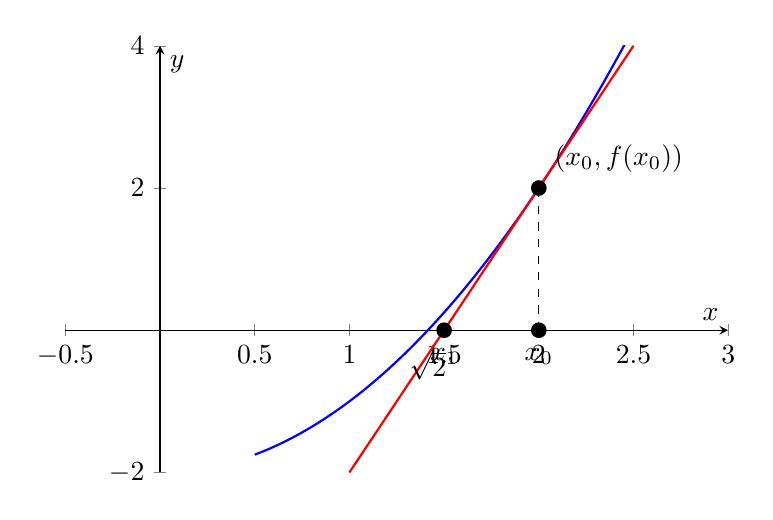
\begin{tikzpicture}
\begin{axis}[
    axis lines=middle,
    xlabel=$x$,
    ylabel=$y$,
    xmin=-0.5, xmax=3,
    ymin=-2, ymax=4,
    width=10cm,
    height=7cm
]
\addplot[blue, thick, domain=0.5:2.5, samples=50] {x^2 - 2};
\addplot[red, thick, domain=1:2.5] {2*2*(x-2) + 2};
\node[circle,fill=black,inner sep=2pt,label={below:$x_0$}] at (axis cs:2,0) {};
\node[circle,fill=black,inner sep=2pt,label={above right:$(x_0, f(x_0))$}] at (axis cs:2,2) {};
\node[circle,fill=black,inner sep=2pt,label={below:$x_1$}] at (axis cs:1.5,0) {};
\draw[dashed] (axis cs:2,0) -- (axis cs:2,2);
\node at (axis cs:1.414,-0.5) {$\sqrt{2}$};
\end{axis}
\end{tikzpicture}
\end{center}

\subsection{Convergence}

\begin{theorem}[Newton-Raphson Convergence]
If $f$ has a simple root at $r$ and $f''$ is continuous near $r$, then Newton-Raphson converges \textbf{quadratically}:
\[
|x_{n+1} - r| \leq C|x_n - r|^2
\]
for some constant $C$ and $x_0$ sufficiently close to $r$.
\end{theorem}

\begin{keypoint}
Quadratic convergence means the number of correct digits approximately \textbf{doubles} with each iteration.
\end{keypoint}

\begin{example}
Find $\sqrt{2}$ using Newton-Raphson on $f(x) = x^2 - 2$.

\textbf{Solution:}
$f'(x) = 2x$, so the iteration is:
\[
x_{n+1} = x_n - \frac{x_n^2 - 2}{2x_n} = \frac{x_n^2 + 2}{2x_n} = \frac{1}{2}\left(x_n + \frac{2}{x_n}\right)
\]

Starting with $x_0 = 1$:
\begin{align*}
x_1 &= \frac{1}{2}(1 + 2) = 1.5\\
x_2 &= \frac{1}{2}(1.5 + 1.333...) = 1.41\overline{6}\\
x_3 &= 1.41421568...\\
x_4 &= 1.41421356237...
\end{align*}

$\sqrt{2} = 1.41421356237...$, so we have 11 correct digits after just 4 iterations!
\end{example}

\begin{warning}
Newton-Raphson can fail if:
\begin{itemize}
    \item $f'(x_n) = 0$ (division by zero)
    \item Initial guess is too far from the root
    \item The function has inflection points or local extrema near the root
\end{itemize}
\end{warning}

%-----------------------------------------------------------------------------
\section{Secant Method}
%-----------------------------------------------------------------------------

\subsection{Derivation}

When the derivative is difficult or expensive to compute, approximate it using a finite difference.

\begin{definition}[Secant Method]
Replace $f'(x_n)$ in Newton-Raphson with a difference quotient:
\[
x_{n+1} = x_n - f(x_n) \cdot \frac{x_n - x_{n-1}}{f(x_n) - f(x_{n-1})}
\]
Requires two initial guesses $x_0$ and $x_1$.
\end{definition}

\subsection{Convergence}

\begin{property}[Secant Convergence]
The secant method converges \textbf{superlinearly} with order $\phi = \frac{1+\sqrt{5}}{2} \approx 1.618$ (the golden ratio):
\[
|x_{n+1} - r| \leq C|x_n - r|^\phi
\]
\end{property}

\begin{keypoint}
The secant method:
\begin{itemize}
    \item Converges faster than bisection but slower than Newton-Raphson
    \item Requires only one function evaluation per iteration (vs. two for Newton-Raphson: $f$ and $f'$)
    \item May diverge if initial guesses are poor
\end{itemize}
\end{keypoint}

%-----------------------------------------------------------------------------
\section{Fixed-Point Iteration}
%-----------------------------------------------------------------------------

\subsection{Theory}

\begin{definition}[Fixed Point]
A \textbf{fixed point} of function $g$ is a value $r$ such that $g(r) = r$.
\end{definition}

To solve $f(x) = 0$, rewrite as $x = g(x)$ for some function $g$.

\begin{definition}[Fixed-Point Iteration]
Starting from $x_0$, compute:
\[
x_{n+1} = g(x_n)
\]
\end{definition}

\begin{theorem}[Fixed-Point Convergence]
If $g$ is continuous on $[a, b]$, $g([a,b]) \subseteq [a,b]$, and $|g'(x)| \leq L < 1$ for all $x \in (a, b)$, then:
\begin{enumerate}
    \item There exists a unique fixed point $r$ in $[a, b]$
    \item For any $x_0 \in [a, b]$, the iteration converges to $r$
    \item $|x_n - r| \leq L^n|x_0 - r|$
\end{enumerate}
\end{theorem}

\begin{example}
Solve $x = \cos(x)$.

Using fixed-point iteration $x_{n+1} = \cos(x_n)$ with $x_0 = 0.5$:
\begin{align*}
x_1 &= \cos(0.5) = 0.8776\\
x_2 &= \cos(0.8776) = 0.6390\\
x_3 &= \cos(0.6390) = 0.8027\\
&\vdots\\
x_{67} &= 0.7390851332...
\end{align*}

The fixed point is $r \approx 0.7390851332$.
\end{example}

\begin{warning}
The choice of $g(x)$ matters! Different rearrangements of $f(x) = 0$ give different convergence behavior. Always verify that $|g'(x)| < 1$ near the root.
\end{warning}

%=============================================================================
%=============================================================================
\chapter{Interpolation}
%=============================================================================
%=============================================================================

\section{Introduction}

\begin{definition}[Interpolation]
Given data points $(x_0, y_0), (x_1, y_1), \ldots, (x_n, y_n)$, \textbf{interpolation} finds a function $P(x)$ that passes through all points:
\[
P(x_i) = y_i \quad \text{for } i = 0, 1, \ldots, n
\]
\end{definition}

%-----------------------------------------------------------------------------
\section{Lagrange Interpolation}
%-----------------------------------------------------------------------------

\begin{theorem}[Lagrange Interpolating Polynomial]
Given $n+1$ distinct points $(x_0, y_0), \ldots, (x_n, y_n)$, there exists a unique polynomial of degree at most $n$:
\[
P_n(x) = \sum_{i=0}^{n} y_i L_i(x)
\]
where the \textbf{Lagrange basis polynomials} are:
\[
L_i(x) = \prod_{j=0, j\neq i}^{n} \frac{x - x_j}{x_i - x_j}
\]
\end{theorem}

\begin{property}[Lagrange Basis Properties]
\[
L_i(x_j) = \begin{cases} 1 & \text{if } i = j \\ 0 & \text{if } i \neq j \end{cases} = \delta_{ij}
\]
\end{property}

\begin{example}
Find the interpolating polynomial through $(0, 1)$, $(1, 3)$, $(2, 2)$.

\textbf{Solution:}
\begin{align*}
L_0(x) &= \frac{(x-1)(x-2)}{(0-1)(0-2)} = \frac{(x-1)(x-2)}{2}\\
L_1(x) &= \frac{(x-0)(x-2)}{(1-0)(1-2)} = \frac{x(x-2)}{-1} = -x(x-2)\\
L_2(x) &= \frac{(x-0)(x-1)}{(2-0)(2-1)} = \frac{x(x-1)}{2}
\end{align*}

\begin{align*}
P_2(x) &= 1 \cdot \frac{(x-1)(x-2)}{2} + 3 \cdot (-x)(x-2) + 2 \cdot \frac{x(x-1)}{2}\\
&= \frac{x^2 - 3x + 2}{2} - 3x^2 + 6x + x^2 - x\\
&= -\frac{3}{2}x^2 + \frac{7}{2}x + 1
\end{align*}
\end{example}

%-----------------------------------------------------------------------------
\section{Newton's Divided Differences}
%-----------------------------------------------------------------------------

\begin{definition}[Divided Differences]
The \textbf{divided differences} are defined recursively:
\begin{align*}
f[x_i] &= f(x_i) = y_i\\
f[x_i, x_{i+1}] &= \frac{f[x_{i+1}] - f[x_i]}{x_{i+1} - x_i}\\
f[x_i, x_{i+1}, \ldots, x_{i+k}] &= \frac{f[x_{i+1}, \ldots, x_{i+k}] - f[x_i, \ldots, x_{i+k-1}]}{x_{i+k} - x_i}
\end{align*}
\end{definition}

\begin{formula}
\textbf{Newton's Interpolating Polynomial:}
\[
P_n(x) = f[x_0] + f[x_0, x_1](x-x_0) + f[x_0, x_1, x_2](x-x_0)(x-x_1) + \cdots
\]
or more compactly:
\[
P_n(x) = \sum_{k=0}^{n} f[x_0, x_1, \ldots, x_k] \prod_{j=0}^{k-1}(x - x_j)
\]
\end{formula}

\begin{example}
Construct the divided difference table for $(0, 1)$, $(1, 3)$, $(2, 2)$, $(3, 5)$.

\begin{center}
\begin{tabular}{c|c|c|c|c}
$x_i$ & $f[x_i]$ & $f[\cdot,\cdot]$ & $f[\cdot,\cdot,\cdot]$ & $f[\cdot,\cdot,\cdot,\cdot]$ \\
\hline
0 & 1 & & & \\
  &   & $\frac{3-1}{1-0}=2$ & & \\
1 & 3 &  & $\frac{-1-2}{2-0}=-\frac{3}{2}$ & \\
  &   & $\frac{2-3}{2-1}=-1$ &  & $\frac{\frac{5}{2}-(-\frac{3}{2})}{3-0}=\frac{4}{3}$ \\
2 & 2 &  & $\frac{3-(-1)}{3-1}=\frac{5}{2}$ & \\
  &   & $\frac{5-2}{3-2}=3$ & & \\
3 & 5 & & & \\
\end{tabular}
\end{center}

Thus:
\[
P_3(x) = 1 + 2x - \frac{3}{2}x(x-1) + \frac{4}{3}x(x-1)(x-2)
\]
\end{example}

%-----------------------------------------------------------------------------
\section{Interpolation Error}
%-----------------------------------------------------------------------------

\begin{theorem}[Interpolation Error]
If $f \in C^{n+1}[a,b]$ and $P_n$ interpolates $f$ at $x_0, \ldots, x_n \in [a,b]$, then for any $x \in [a,b]$:
\[
f(x) - P_n(x) = \frac{f^{(n+1)}(\xi)}{(n+1)!} \prod_{i=0}^{n}(x - x_i)
\]
for some $\xi$ between the smallest and largest of $x, x_0, \ldots, x_n$.
\end{theorem}

\begin{warning}
\textbf{Runge's Phenomenon:} High-degree polynomial interpolation with equally spaced points can lead to wild oscillations near the endpoints. Using Chebyshev nodes helps mitigate this.
\end{warning}

%=============================================================================
%=============================================================================
\chapter{Numerical Differentiation and Integration}
%=============================================================================
%=============================================================================

\section{Numerical Differentiation}

\subsection{Finite Difference Formulas}

\begin{formula}
\textbf{Forward Difference:}
\[
f'(x) \approx \frac{f(x+h) - f(x)}{h} + O(h)
\]

\textbf{Backward Difference:}
\[
f'(x) \approx \frac{f(x) - f(x-h)}{h} + O(h)
\]

\textbf{Central Difference:}
\[
f'(x) \approx \frac{f(x+h) - f(x-h)}{2h} + O(h^2)
\]
\end{formula}

\begin{keypoint}
Central difference is more accurate ($O(h^2)$) than forward or backward difference ($O(h)$), but requires function values on both sides of $x$.
\end{keypoint}

\subsection{Second Derivative}

\begin{formula}
\textbf{Central Difference for Second Derivative:}
\[
f''(x) \approx \frac{f(x+h) - 2f(x) + f(x-h)}{h^2} + O(h^2)
\]
\end{formula}

\begin{warning}
Numerical differentiation is \textbf{ill-conditioned}: small errors in function values get amplified. There's a trade-off between truncation error (decreases with smaller $h$) and round-off error (increases with smaller $h$).
\end{warning}

%-----------------------------------------------------------------------------
\section{Numerical Integration (Quadrature)}
%-----------------------------------------------------------------------------

\subsection{The Basic Problem}

Approximate the definite integral:
\[
I = \int_a^b f(x)\, dx
\]

\subsection{Trapezoidal Rule}

\begin{definition}[Trapezoidal Rule]
Approximate the area under $f$ by a trapezoid:
\[
\int_a^b f(x)\, dx \approx \frac{b-a}{2}[f(a) + f(b)]
\]
\end{definition}

\begin{formula}
\textbf{Composite Trapezoidal Rule:}

Divide $[a, b]$ into $n$ subintervals of width $h = \frac{b-a}{n}$:
\[
\int_a^b f(x)\, dx \approx \frac{h}{2}\left[f(a) + 2\sum_{i=1}^{n-1}f(a + ih) + f(b)\right]
\]

Error: $O(h^2)$
\end{formula}

\subsection{Simpson's Rule}

\begin{definition}[Simpson's Rule]
Use a quadratic polynomial to approximate $f$ over two subintervals:
\[
\int_a^b f(x)\, dx \approx \frac{b-a}{6}\left[f(a) + 4f\left(\frac{a+b}{2}\right) + f(b)\right]
\]
\end{definition}

\begin{formula}
\textbf{Composite Simpson's Rule:}

For $n$ even subintervals with $h = \frac{b-a}{n}$:
\[
\int_a^b f(x)\, dx \approx \frac{h}{3}\left[f(a) + 4\sum_{\text{odd } i}f(x_i) + 2\sum_{\text{even } i}f(x_i) + f(b)\right]
\]

Error: $O(h^4)$
\end{formula}

\begin{example}
Approximate $\int_0^1 e^{-x^2}\, dx$ using Simpson's rule with $n = 4$.

\textbf{Solution:}
$h = 0.25$, points: $x_0 = 0$, $x_1 = 0.25$, $x_2 = 0.5$, $x_3 = 0.75$, $x_4 = 1$

\begin{align*}
f(x_0) &= e^0 = 1\\
f(x_1) &= e^{-0.0625} = 0.9394\\
f(x_2) &= e^{-0.25} = 0.7788\\
f(x_3) &= e^{-0.5625} = 0.5698\\
f(x_4) &= e^{-1} = 0.3679
\end{align*}

\[
I \approx \frac{0.25}{3}[1 + 4(0.9394 + 0.5698) + 2(0.7788) + 0.3679] = 0.7468
\]

(Exact value: $\approx 0.7468$)
\end{example}

\begin{keypoint}
\begin{center}
\begin{tabular}{|c|c|c|}
\hline
\textbf{Method} & \textbf{Degree of Precision} & \textbf{Error} \\
\hline
Midpoint Rule & 1 & $O(h^2)$ \\
Trapezoidal Rule & 1 & $O(h^2)$ \\
Simpson's Rule & 3 & $O(h^4)$ \\
Simpson's 3/8 Rule & 3 & $O(h^4)$ \\
\hline
\end{tabular}
\end{center}
\end{keypoint}

%=============================================================================
%=============================================================================
\chapter{Systems of Linear Equations}
%=============================================================================
%=============================================================================

\section{Introduction}

We seek to solve:
\[
A\mathbf{x} = \mathbf{b}
\]
where $A$ is an $n \times n$ matrix, $\mathbf{x}$ is the unknown vector, and $\mathbf{b}$ is the right-hand side.

%-----------------------------------------------------------------------------
\section{Gaussian Elimination}
%-----------------------------------------------------------------------------

\subsection{Forward Elimination}

Transform the augmented matrix $[A|\mathbf{b}]$ to upper triangular form using row operations.

\begin{algorithmbox}
\textbf{Forward Elimination:}

For $k = 1$ to $n-1$:
\begin{enumerate}
    \item For $i = k+1$ to $n$:
    \begin{enumerate}
        \item Compute multiplier: $m_{ik} = \frac{a_{ik}}{a_{kk}}$
        \item For $j = k$ to $n$: $a_{ij} = a_{ij} - m_{ik} \cdot a_{kj}$
        \item $b_i = b_i - m_{ik} \cdot b_k$
    \end{enumerate}
\end{enumerate}
\end{algorithmbox}

\subsection{Back Substitution}

Solve the upper triangular system:
\begin{align*}
x_n &= \frac{b_n}{a_{nn}}\\
x_i &= \frac{1}{a_{ii}}\left(b_i - \sum_{j=i+1}^{n} a_{ij}x_j\right) \quad \text{for } i = n-1, \ldots, 1
\end{align*}

\begin{example}
Solve:
\[
\begin{cases}
2x + y - z = 8\\
-3x - y + 2z = -11\\
-2x + y + 2z = -3
\end{cases}
\]

Augmented matrix:
\[
\left[\begin{array}{ccc|c}
2 & 1 & -1 & 8\\
-3 & -1 & 2 & -11\\
-2 & 1 & 2 & -3
\end{array}\right]
\]

After forward elimination:
\[
\left[\begin{array}{ccc|c}
2 & 1 & -1 & 8\\
0 & \frac{1}{2} & \frac{1}{2} & 1\\
0 & 0 & -1 & 1
\end{array}\right]
\]

Back substitution: $z = -1$, $y = 3$, $x = 2$
\end{example}

\subsection{Partial Pivoting}

\begin{warning}
If $a_{kk} = 0$ (or very small), Gaussian elimination fails (or becomes unstable). Use \textbf{partial pivoting}: at step $k$, swap rows so that $|a_{kk}|$ is maximized among rows $k, k+1, \ldots, n$.
\end{warning}

%-----------------------------------------------------------------------------
\section{LU Decomposition}
%-----------------------------------------------------------------------------

\begin{definition}[LU Decomposition]
Factor $A$ as $A = LU$ where:
\begin{itemize}
    \item $L$ is lower triangular with 1's on the diagonal
    \item $U$ is upper triangular
\end{itemize}
\end{definition}

\begin{property}[Solving with LU]
To solve $A\mathbf{x} = \mathbf{b}$:
\begin{enumerate}
    \item Factor: $A = LU$ (done once)
    \item Solve $L\mathbf{y} = \mathbf{b}$ (forward substitution)
    \item Solve $U\mathbf{x} = \mathbf{y}$ (back substitution)
\end{enumerate}
\end{property}

\begin{keypoint}
LU decomposition is advantageous when solving multiple systems with the same matrix $A$ but different right-hand sides $\mathbf{b}$.
\end{keypoint}

%-----------------------------------------------------------------------------
\section{Iterative Methods}
%-----------------------------------------------------------------------------

\subsection{Jacobi Method}

\begin{definition}[Jacobi Iteration]
Rewrite $A\mathbf{x} = \mathbf{b}$ as $\mathbf{x} = D^{-1}(\mathbf{b} - (L+U)\mathbf{x})$ where $A = D + L + U$ (diagonal, strictly lower, strictly upper).

Iteration:
\[
x_i^{(k+1)} = \frac{1}{a_{ii}}\left(b_i - \sum_{j \neq i} a_{ij}x_j^{(k)}\right)
\]
\end{definition}

\subsection{Gauss-Seidel Method}

\begin{definition}[Gauss-Seidel Iteration]
Use updated values immediately:
\[
x_i^{(k+1)} = \frac{1}{a_{ii}}\left(b_i - \sum_{j < i} a_{ij}x_j^{(k+1)} - \sum_{j > i} a_{ij}x_j^{(k)}\right)
\]
\end{definition}

\begin{property}[Convergence Conditions]
\begin{itemize}
    \item \textbf{Sufficient:} $A$ is strictly diagonally dominant ($|a_{ii}| > \sum_{j \neq i}|a_{ij}|$)
    \item \textbf{Sufficient:} $A$ is symmetric positive definite (for Gauss-Seidel)
\end{itemize}
\end{property}

%=============================================================================
%=============================================================================
\chapter{Numerical Solutions of ODEs}
%=============================================================================
%=============================================================================

\section{Initial Value Problems}

\begin{definition}[Initial Value Problem (IVP)]
Find $y(t)$ satisfying:
\[
\frac{dy}{dt} = f(t, y), \quad y(t_0) = y_0
\]
\end{definition}

%-----------------------------------------------------------------------------
\section{Euler's Method}
%-----------------------------------------------------------------------------

\begin{definition}[Euler's Method]
The simplest numerical method for ODEs:
\[
y_{n+1} = y_n + h \cdot f(t_n, y_n)
\]
where $h$ is the step size and $t_n = t_0 + nh$.
\end{definition}

\begin{center}
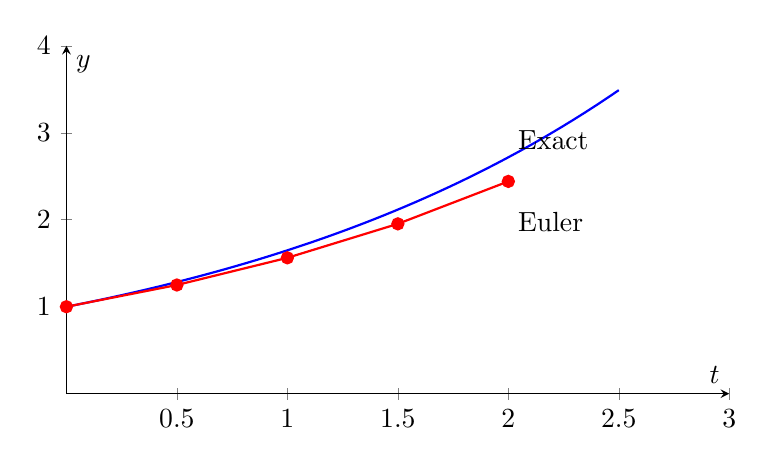
\begin{tikzpicture}
\begin{axis}[
    axis lines=middle,
    xlabel=$t$,
    ylabel=$y$,
    xmin=0, xmax=3,
    ymin=0, ymax=4,
    width=10cm,
    height=6cm
]
\addplot[blue, thick, domain=0:2.5, samples=50] {exp(x/2)};
\addplot[red, thick, mark=*] coordinates {(0,1) (0.5,1.25) (1,1.5625) (1.5,1.953) (2,2.441)};
\node[above right] at (axis cs:2,2.7) {Exact};
\node[below right] at (axis cs:2,2.2) {Euler};
\end{axis}
\end{tikzpicture}
\end{center}

\begin{property}[Euler's Method Error]
\begin{itemize}
    \item \textbf{Local truncation error}: $O(h^2)$
    \item \textbf{Global error}: $O(h)$
\end{itemize}
Euler's method is \textbf{first-order accurate}.
\end{property}

\begin{example}
Solve $y' = y$, $y(0) = 1$ on $[0, 1]$ with $h = 0.2$.

\textbf{Solution:} Exact solution: $y = e^t$

\begin{center}
\begin{tabular}{|c|c|c|c|}
\hline
$n$ & $t_n$ & $y_n$ (Euler) & $y(t_n)$ (Exact) \\
\hline
0 & 0.0 & 1.0000 & 1.0000 \\
1 & 0.2 & 1.2000 & 1.2214 \\
2 & 0.4 & 1.4400 & 1.4918 \\
3 & 0.6 & 1.7280 & 1.8221 \\
4 & 0.8 & 2.0736 & 2.2255 \\
5 & 1.0 & 2.4883 & 2.7183 \\
\hline
\end{tabular}
\end{center}
\end{example}

%-----------------------------------------------------------------------------
\section{Runge-Kutta Methods}
%-----------------------------------------------------------------------------

\subsection{Second-Order (Midpoint Method)}

\begin{formula}
\textbf{Midpoint Method (RK2):}
\begin{align*}
k_1 &= h \cdot f(t_n, y_n)\\
k_2 &= h \cdot f\left(t_n + \frac{h}{2}, y_n + \frac{k_1}{2}\right)\\
y_{n+1} &= y_n + k_2
\end{align*}
\end{formula}

\subsection{Fourth-Order (Classical RK4)}

\begin{formula}
\textbf{Classical Runge-Kutta (RK4):}
\begin{align*}
k_1 &= h \cdot f(t_n, y_n)\\
k_2 &= h \cdot f\left(t_n + \frac{h}{2}, y_n + \frac{k_1}{2}\right)\\
k_3 &= h \cdot f\left(t_n + \frac{h}{2}, y_n + \frac{k_2}{2}\right)\\
k_4 &= h \cdot f(t_n + h, y_n + k_3)\\
y_{n+1} &= y_n + \frac{1}{6}(k_1 + 2k_2 + 2k_3 + k_4)
\end{align*}
\end{formula}

\begin{property}[RK4 Error]
\begin{itemize}
    \item \textbf{Local truncation error}: $O(h^5)$
    \item \textbf{Global error}: $O(h^4)$
\end{itemize}
RK4 is \textbf{fourth-order accurate}.
\end{property}

\begin{keypoint}
RK4 is the workhorse of numerical ODE solving:
\begin{itemize}
    \item Good balance of accuracy and computational cost
    \item Four function evaluations per step
    \item Very accurate for smooth problems
\end{itemize}
\end{keypoint}

\begin{example}
Solve $y' = -2ty$, $y(0) = 1$ using RK4 with $h = 0.1$ at $t = 0.1$.

\textbf{Solution:} $f(t, y) = -2ty$

\begin{align*}
k_1 &= 0.1 \cdot (-2)(0)(1) = 0\\
k_2 &= 0.1 \cdot (-2)(0.05)(1) = -0.01\\
k_3 &= 0.1 \cdot (-2)(0.05)(0.995) = -0.00995\\
k_4 &= 0.1 \cdot (-2)(0.1)(0.99005) = -0.0198
\end{align*}

\[
y_1 = 1 + \frac{1}{6}(0 - 0.02 - 0.0199 - 0.0198) = 0.99005
\]

Exact: $y = e^{-t^2}$, so $y(0.1) = e^{-0.01} = 0.99005$
\end{example}

%=============================================================================
\chapter*{Summary}
\addcontentsline{toc}{chapter}{Summary}
%=============================================================================

\section*{Chapter 1: Errors}
\begin{itemize}
    \item Absolute error: $|x - \tilde{x}|$; Relative error: $\frac{|x - \tilde{x}|}{|x|}$
    \item Sources: round-off, truncation, input, human
    \item Avoid catastrophic cancellation in subtraction
\end{itemize}

\section*{Chapter 2: Root Finding}
\begin{itemize}
    \item Bisection: robust, linear convergence $O(1/2^n)$
    \item Newton-Raphson: $x_{n+1} = x_n - \frac{f(x_n)}{f'(x_n)}$, quadratic convergence
    \item Secant: superlinear convergence, no derivative needed
    \item Fixed-point: $x_{n+1} = g(x_n)$, converges if $|g'(r)| < 1$
\end{itemize}

\section*{Chapter 3: Interpolation}
\begin{itemize}
    \item Lagrange: $P_n(x) = \sum y_i L_i(x)$
    \item Newton: divided differences, efficient for adding points
    \item Error: $\frac{f^{(n+1)}(\xi)}{(n+1)!}\prod(x-x_i)$
    \item Beware of Runge's phenomenon
\end{itemize}

\section*{Chapter 4: Differentiation and Integration}
\begin{itemize}
    \item Central difference: $f'(x) \approx \frac{f(x+h)-f(x-h)}{2h}$, $O(h^2)$
    \item Trapezoidal: $\frac{h}{2}[f(a) + 2\sum f(x_i) + f(b)]$, $O(h^2)$
    \item Simpson's: $\frac{h}{3}[f + 4\sum_{\text{odd}} + 2\sum_{\text{even}}]$, $O(h^4)$
\end{itemize}

\section*{Chapter 5: Linear Systems}
\begin{itemize}
    \item Gaussian elimination with partial pivoting: $O(n^3)$
    \item LU decomposition: efficient for multiple right-hand sides
    \item Jacobi/Gauss-Seidel: iterative, good for large sparse systems
\end{itemize}

\section*{Chapter 6: ODEs}
\begin{itemize}
    \item Euler: $y_{n+1} = y_n + hf(t_n, y_n)$, first-order
    \item RK4: fourth-order, excellent accuracy/cost ratio
    \item Step size choice balances accuracy vs. stability
\end{itemize}

\end{document}
